% !TEX root = ../../semexp-thesis.tex

\section{The Semantic Workspace}
\label{sec:approach/workspace}

To study our concept of an augmented exploratory programming workflow, we describe the \emph{semantic workspace} as a conceptual framework for semantic exploratory programming systems that contains different \emph{semantic exploratory programming tools}.
Within this framework, we investigate different manifestations of the augmented exploratory programming workflow through semantic tools that support programmers at different levels at abstraction in their research process and combine different types of semantic interfaces.

\begin{figure}
	\centering
	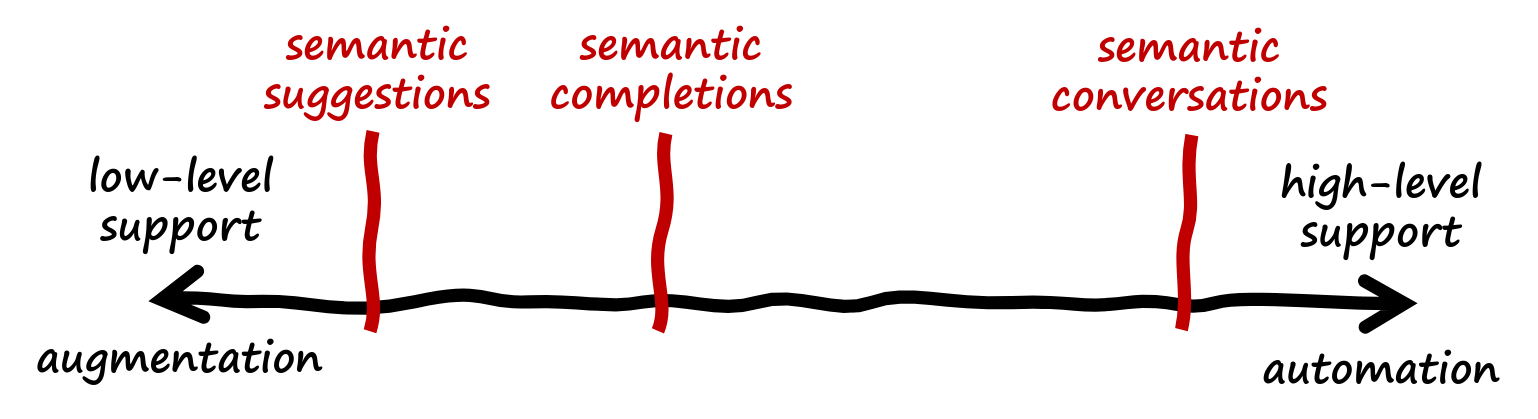
\includegraphics[width=.85\textwidth]{02_workspace/spectrum.png}
	\caption[The support spectrum of different \emph{semantic tools} in the semantic workspace.]{
		The support spectrum of different tools in the semantic workspace.
		Low-level semantic tools collect context from tracking the actions of programmers in the programming system and \emph{augment} their exploration through new suggestions.
		High-level semantic tools retrieve explicit conceptual descriptions from programmers and \emph{automate} a larger part of the research process.
	}
	\label{fig:approach/workspace/spectrum}
\end{figure}

All of those manifestations can be arranged in a spectrum based on their degree of support between two extremes~(\cref{fig:approach/workspace/spectrum}):

\begin{description}
	\item[Augmentation:]
	The one extreme of the spectrum contains tools that operate at a lower level of abstraction and provide narrow support to programmers.
	Low-level semantic tools primarily employ technical interfaces and artifacts such as experiments and \emph{augment} the research process of programmers by providing suggestions for smaller parts of their workflow, such as other experiments.

	\item[Automation:]
	The other extreme contains tools that provide wide-ranging, more conceptual semantic support.
	In contrast to low-level semantic tools, they often employ new semantic interfaces to exchange conceptual artifacts with programmers.
	Rather than augmenting the exploratory programming workflow, they tend to \emph{automate} parts of it and provide programmers with aggregated results and answers instead of low-level suggestions.
\end{description}

Orthogonally to their degree of support, semantic tools can offer either reactive or proactive interaction mechanisms:
reactive tools will expect an explicit question or invocation by the programmer, while proactive tools will observe the steps of programmers in the background and make suggestions before a programmer explicitly requests support.
Similar to the degree of support, semantic tools can combine characteristics of either interaction mechanisms.

The choice between augmenting and automating or reactive and proactive semantic tools relates to the current objectives of programmers and has different implications on their overall programming experience, trust, and learning curve, which we will discuss in \cref{cha:discussion}. % todo: is this forward reference good style?

In the semantic workspace, we propose three concepts for novel semantic tools that can be added on top of traditional exploratory programming systems and that together provide different means for exploratory programmers to augment and partially automate their workflow:

\begin{description}[noextralabelsep]
	\item[Semantic suggestions] anticipate the plans of programmers by continuously monitoring their experimental activities and proactively suggesting further experiments as well as optional summaries.
	\item[Semantic completions] monitor the planning activities of programmers as they draft code or text in editors, automatically generate and conduct experiments, and proactively provide contextualized suggestions such as code snippets in the editor.
	\item[Semantic conversations] provide an interface through that programmers can express conceptual questions about objects (such as domain objects or classes) in natural language and retrieve answers at the same abstraction level.
	Internally, an exploratory programming agent conducts the necessary plans, experiments, and deductions to generate answers.
\end{description}
In the following, we describe each semantic tool concept in detail.

\subsection{Semantic Suggestions}
\label{sec:approach/workspace/suggestions}

\begin{figure}
	\centering
	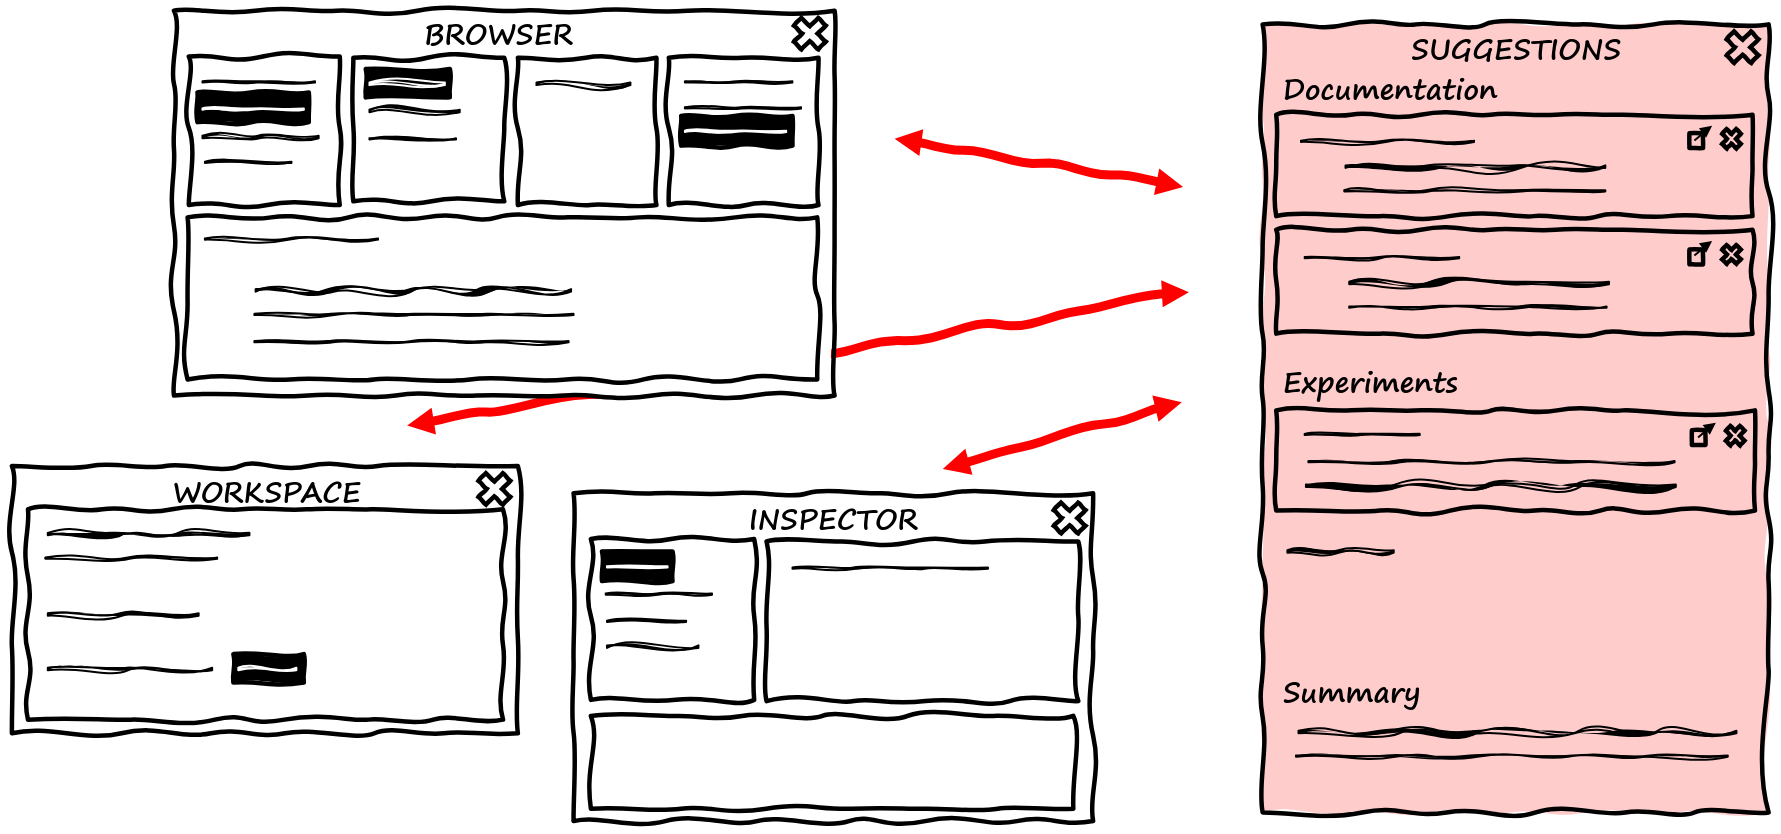
\includegraphics[width=\textwidth]{02_workspace/suggestions.png}
	\caption[Our concept of a \emph{semantic suggestions} tool in the semantic workspace.]{
		Our concept of a \emph{semantic suggestions} tool in the semantic workspace.
		The augmented programming system tracks the experimental actions of the programmer through traditional programming tools (\bold{\textcolor{gray}{gray}}), anticipates the possible next steps of the programmer, and provides them with a list of suggestions for further experiments as well as an optional summary of their results (\bold{\textcolor{red}{red}}).
	}
	\label{fig:approach/workspace/suggestions}
\end{figure}

The approach of \emph{semantic suggestions} is to augment the research process of exploratory programmers by providing them with possible experiments based on their previous experimental activities.
For this, the semantic workspace tracks the experiments that programmers execute through the interfaces of traditional exploratory programming systems such as do-its, code browsers, and method finders.
Based on these observed experiments, it attempts to reconstruct the plans of programmers such as an intention to understand the (scattered) implementation of a concept or to develop a new prototype for a user interface.
Using this reconstructed plan, the semantic workspace then generates further possibly relevant experiments and suggests them to the programmer.

Suggestions are proactively generated and presented in a list-like interface such as a dock that is placed next to other tools in the system through which programmers conduct experiments~(\cref{fig:approach/workspace/suggestions}).
%Suggested experiments typically revolve around research activities such as browing code or documentation.

Semantic suggestions exploit the ability of semantic technologies to process information at a larger scale than human beings, even though with a reduced precision and recall.
For this reason, the number of generated suggestions is usually in the two- to three-digit range.
This necessitates a structured and ranked presentation of suggestions, which is achieved by grouping them based on their type (such as classes versus methods) and ranking them based on their relevance, similarity, and diversity~(see \cref{sec:suggestions/ranking}).

Optionally, semantic suggestions can include summaries and deduced results of all experiments.
For example, the central aspects from a complex implementation or lengthy documentation could be briefly summarized in the context of the anticipated plans of programmers as a natural-language synopsis.

Semantic suggestions can be applied for different types of plans and experimental activities, including but not limited to the following use cases:

%\begin{description}
	%\item[Code browsing:]
	\paragraph{Code browsing}
	To understand the implementation of a concept, a programmer is reading one or multiple methods through traditional code browsers.
	The semantic workspace anticipates the likely intention of understanding a concept and thus suggests further methods and code artifacts that the programmer might want to browse next.
	This includes:

	\begin{description}[noextralabelsep]
		\item[senders] of the currently viewed methods: methods that (possibly) invoke the current methods~(see \cref{par:background/expsys/tools/browsing});
		\item[implementors] of messages that the current methods send, displayed with their comment and implementation;
		\item[classes] that the current methods reference, displayed with their comment and definition;
		\item[similar methods,] e.g., methods that pursue the same goal or implement common strategies.
	\end{description}
	%senders of the currently viewed methods (i.e., methods that possibly invoke the former methods, see \cref{par:background/expsys/tools/browsing}), the comment and implementation of messages that the current methods send, the comment and definition of classes that the current methods reference, \emph{similar} methods (e.g., methods that pursue the same goal or include common strategies)

	\noindent
	Beyond code artifacts, the system could also suggest other types of semantic suggestions in this context such as relevant excerpt from related documentation artifacts, design documents, or specifications.

	Depending on the quantity and complexity of related artifacts, the system might also summarize all suggestions, e.g., by describing the implementation of a scattered concept or shortening and paraphrasing documentation artifacts.

	%\item[Prototyping:]
	\paragraph{Prototyping}
	While programmers write and repeatedly save a new method as part of creating a prototype, the semantic workspace anticipates the type and shape of desired prototype.
	To support this activity, it provides the programmer with possibly relevant suggestions for related resources:

	\begin{description}[noextralabelsep]
		\item[similar methods,] e.g., methods that pursue the same goal or implement similar strategies to the current unfinished method;
		\item[correlated methods and classes] that are used by those similar methods and that the programmer thus might consider to use in the current prototype method as well (resembling the concept of collaborative filtering, i.e., ``programmers who have sent this message have also sent that message''), displayed with their comment and usage samples;
		\item[documentation artifacts] that describe the concept and intended usage of present and suggested classes and methods.
	\end{description}

	%\item[Debugging:]
	\paragraph{Debugging}
	Semantic suggestions can support programmers who are experiencing an error while using the software system and are investigating it in a debugger to understand its causes and solve it.
	%To this end, the semantic workspace automatically searches bug trackers or other communication platforms of developers for references of the same error message, browses available documentation artifacts, or finds related exception handlers in the software system.
	To this end, the semantic workspace automatically searches different sources to provide several types of suggestions:

	\begin{description}[noextralabelsep]
		\item[bug reports] on bug trackers or other communication platforms that refer to the same error message;
		\item[documentation artifacts] that describe causes or solutions for this error;
		\item[exception handlers] for this and similar errors in the software system.
	\end{description}

	\noindent
	%This information is prepared and provided to the programmer to provide starting points for further research.
	Additionally, the system might also summarize the results to extract and suggest particular debugging and solution strategies (such as checking the state of an object, initializing a resource, or inserting a missing exception handler).

	% todo: müssen mal schauen, ob wir hier zu viel details von retrieval vorwegnehmen. einerseits sind wir schon ziemlich detailliert, andererseits technisch gesehen nicht vollständig (z. b. tests, global bindings, type of documetnation artifacts).
%\end{description}

\ParSep

Thus, semantic suggestions support exploratory programmers in their research process by providing them with further possible experiments and automated deductions of them.
This does not only accelerate particular research activities but also augments the insights of programmers as they can gain inspiration from suggestions that would otherwise not have come to their mind or would have been associated with too high manual research cost.

\subsection{Semantic Completions}
\label{sec:approach/workspace/completions}

Similarly to semantic suggestions, \emph{semantic completions} observe the activity of programmers in the system and proactively provide them with further contextually relevant suggestions.
However, semantic completions support programmers at higher levels of abstraction in their research process:
instead of tracking manual experiments of programmers and reconstructing their possible plans from these, semantic completions exploit existing interfaces of exploratory programming systems through that programmers can express their plans, and create an image of these plans directly.
Concretely, these interfaces involve different types of editors through that programmers create and edit text, code, or domain-specific objects.
The semantic workspace does not wait until the programmer finishes their input and submits it to the system but tracks their editing activity continuously (e.g., as they type or click) to follow along their plans.

\begin{figure}
	\centering
	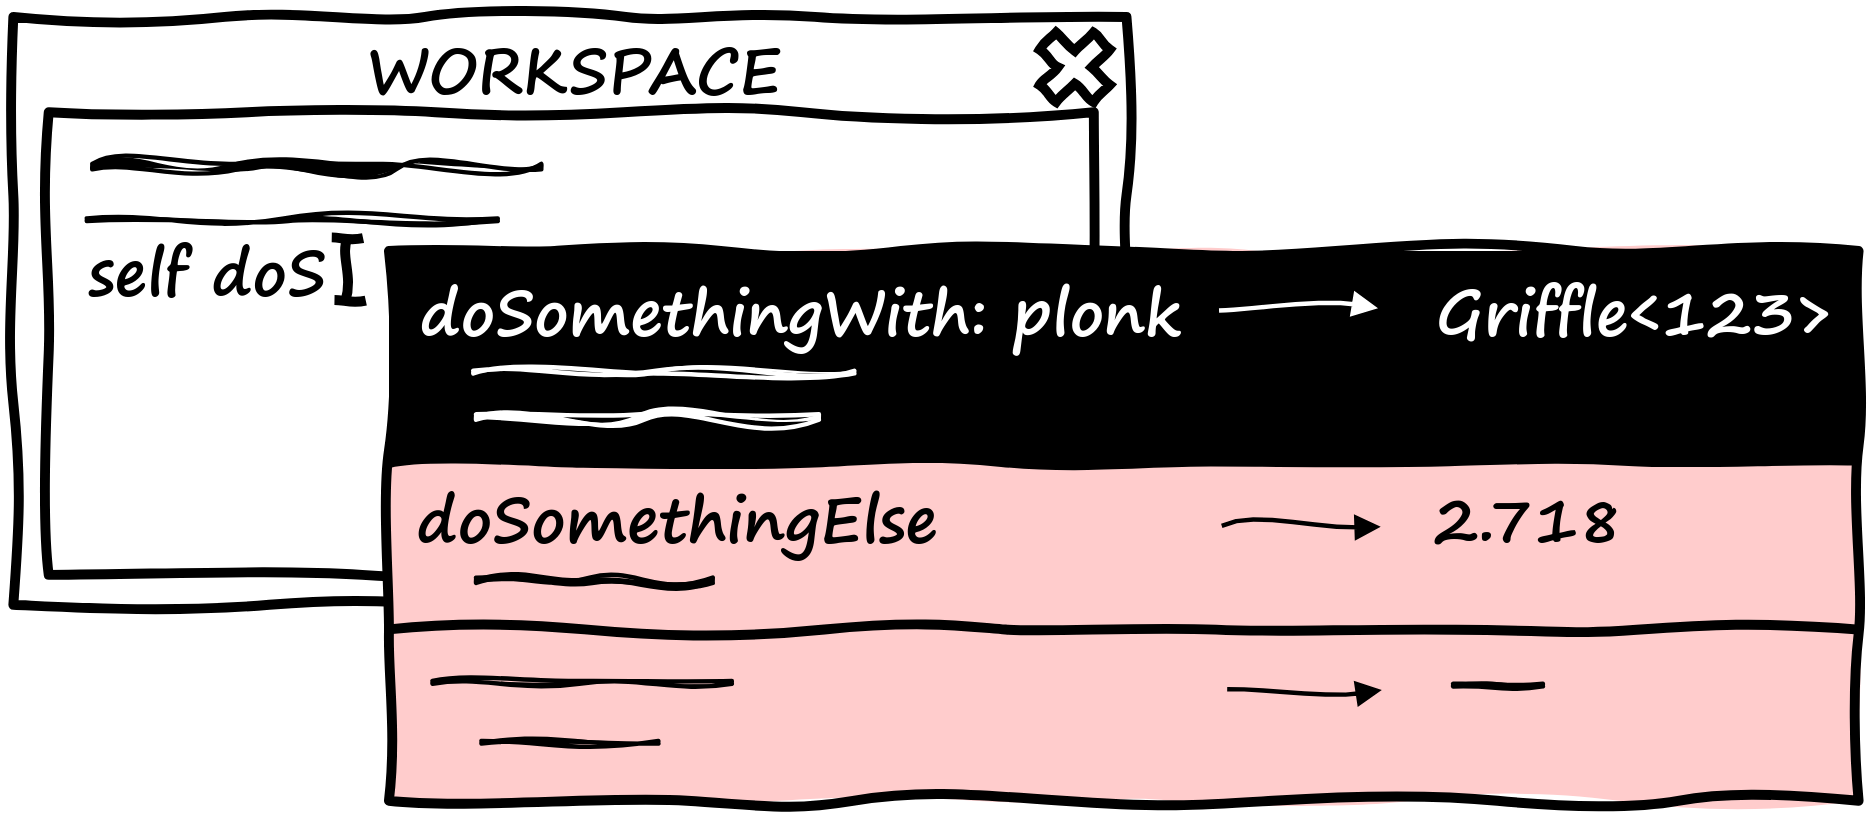
\includegraphics[width=0.58\textwidth]{02_workspace/completions.png}
	\caption[Our concept of a \emph{semantic completions} tool in the semantic workspace.]{
		Our concept of a \emph{semantic completions} tool in the semantic workspace.
		While programmers gradually express their plan to the system, e.g., by drafting a script in a traditional workspace (\bold{\textcolor{gray}{gray}}), the augmented programming system reconstructs their underlying intentions and suggests them contextualized experiments as completions of their existing inputs (\bold{\textcolor{red}{red}}).
	}
	\label{fig:approach/workspace/completions}
\end{figure}

Feedback of semantic completions is provided to programmers through conceptual, highly contextualized results instead of single experiment suggestions.
This manifests as a list of completions that are integrated into the editor interface and that represent possible continuations of the preliminary plan that programmers have typed into the editor before.

To generate these completions, the semantic workspace internally predicts, executes, and evaluates possible experiments of programmers based on their observed plans in a similar manner to semantic suggestions.
After that, results are filtered, aggregated, and transformed into the input context of the programmer.

Semantic completions can be applied to different types of planning activities that exploratory programmers conduct as part of their research process, for example:

\paragraph{Prototyping}
While programmers write or edit the code of a script or method (e.g., through a textual or visual editor), the system observes their activity and derives their plans.
It automatically researches similar methods, correlated class and method names, and relevant documentation artifacts.
Based on this information, it synthetizes possible code snippets (that may range from single expressions to entire methods) and suggests them as contextually adjusted completions to the programmer in their editor.

Optionally, these contextualized suggestions can also be dynamically enriched.
For example, the system can present a completed code expression together with the result of evaluating it (using available context such as call stacks, Babylonian examples, or symbolic execution, see %\crefrange{par:background/expsys/tools/debugging}{par:background/expsys/tools/symbex}
\cref{sec:background/expsys/tools}%
) or display the effect of a completed method, such as a preview of a graphical prototype.

% todo: concrete example here?

\paragraph{Natural-language communication}
% todo: find better name for this? documentation? human-to-human communication?
Another frequent activity of programmers regards to writing messages for human communication with other programmers, such as documentation artifacts, bug reports, and commit messages.
This can be considered as another type of plans and experiments that programmers conduct to express their intentions to the system and benefit from the outputs of the system (e.g., through answers to their questions from other programmers or through reminders to their ``future selves'' about their original intentions)\footnote{This perspective can also apply to source code which ``must be written for people to read,
and only incidentally for machines to execute''~\cite[p.~xxii]{abelson1996structure}.}.

Semantic completions can assist programmers with writing such natural-language text by automatically browsing and suggesting relevant classes, methods, or other artifacts such as bug reports and commits, generating example experiments, and completing the sentences started by programmers to fill in this information.
For example, when a programmer creates a bug report, the system could automatically summarize prior notes and experiments from other workspaces into a consolidated text and insert a test to reproduce the bug.

\ParSep

Thus, semantic completions can support programmers in creating and realizing plans by directly following their intentions, generating and conducting likely experiments, and contributing insights from them to the programmers' planning activity in a contextualized form.
This allows programmers to interact with the programming system at a more conceptual level, accelerate their workflow for trivial tasks, and explore different solutions based on an extended, diverse amount of information.

% todo: fehlt uns hier noch offensichtliches?

\subsection{Semantic Conversations}
\label{sec:approach/workspace/conversations}

\emph{Semantic conversations} support exploratory programmers at a high abstraction level in their research process.
For this, a programmer can ask a conceptual question about the software system, and the semantic workspace will return an answer to that question in a similar conceptual, natural-language form~(\cref{fig:approach/workspace/conversation}).
The programmer can ask follow-up questions based on an answer by the system, and the system may also ask questions back to the programmer to clarify questions, resulting in a conversational interaction style.

\begin{figure}
	\centering
	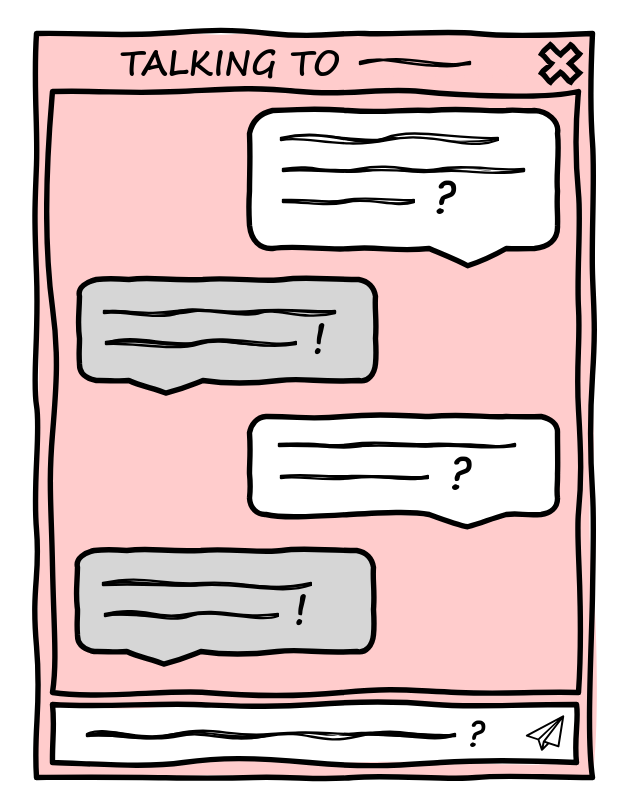
\includegraphics[width=0.35\textwidth]{02_workspace/conversation.png}
	\caption[Our concept of a \emph{semantic conversations} tool in the semantic workspace.]{
		Our concept of a \emph{semantic conversations} tool in the semantic workspace.
		Programmers express their abstract, contextual questions to the augmented programming system by interacting with an object in the software system through messages in natural language.
		Internally, the programming system conducts all steps of the required research process for answering the questions autonomously and returns an abstract, natural-language answer to the programmer.
	}
	\label{fig:approach/workspace/conversation}
\end{figure}

Internally, the system executes an entire instance of the (potentially nested) research process on its own: it generates a plan to answer the question, generates, executes, and analyzes one or several experiments, repeats as necessary, and finally creates an answer to the question based on the gained results.

Following the object-oriented philosophy of many exploratory programming systems such as Smalltalk systems, we define one reference object from the system for each semantic conversation.
Thus, just like programmers can send messages to objects through inspect and interact with them, they can also ask them natural-language questions through semantic conversations.

\begin{example}
	A programmer inspects an order object from a shopping system and wants to know when the order was created.
	To find this out, they ask the object ``when were you created'' through a conversational interface.
	In response, the system internally conducts multiple experiments to explore the inner structure and protocols of the order's class, inspect the internal state of the order object or send messages to it, and run further scripts to convert a retrieved value into a proper format.
	Finally, the system answers the question of the programmer with an answer like: ``I was created at March 14th this year.''
\end{example}

Reference objects can be arbitrary objects from the system, ranging from domain objects over code objects such as classes and methods to derived artifacts of software systems such as test results, program traces, and views from other tools.

Thus, semantic conversations provide an abstract, reactive interface through that programmers can express questions about objects and communicate with the system in natural language.
This allows them to avoid context switches and distractions and handle overarching research processes more efficiently.
At the same time, the system is able to process more information than the programmer within the same time, creating a chance to provide them with a more extensive overview of a part of the software system within a single conversation.
